\documentclass[12pt,twoside]{report}
\makeatletter
\def\@makechapterhead#1{%
  \vspace*{1\p@}%
  {\parindent \z@ \raggedright \normalfont
    \interlinepenalty\@M
    \Huge\bfseries  \thechapter.\quad #1\par\nobreak
    \vskip 40\p@
  }}
\makeatother
\usepackage[utf8]{inputenc}
\usepackage{graphicx}
\usepackage{caption}
\usepackage{subcaption}
\usepackage[a4paper,width=150mm,top=25mm,bottom=25mm,bindingoffset=6mm]{geometry}
\usepackage{fancyhdr}
\pagestyle{fancy}
\fancyhead{}
\fancyhead[L]{Group 12 Managment Report}
\fancyfoot{}
\fancyfoot[R]{\thepage}
\renewcommand{\headrulewidth}{0.4pt}
\renewcommand{\footrulewidth}{0.4pt}
\usepackage{listings}
\usepackage{color}
\usepackage[numbers]{natbib}
\usepackage{float}







\definecolor{dkgreen}{rgb}{0,0.6,0}
\definecolor{gray}{rgb}{0.5,0.5,0.5}
\definecolor{mauve}{rgb}{0.58,0,0.82}

\lstset{frame=tb,
  language=Java,
  aboveskip=3mm,
  belowskip=3mm,
  showstringspaces=false,
  columns=flexible,
  basicstyle={\small\ttfamily},
  numbers=none,
  numberstyle=\tiny\color{gray},
  keywordstyle=\color{blue},
  commentstyle=\color{dkgreen},
  stringstyle=\color{mauve},
  breaklines=true,
  breakatwhitespace=true,
  tabsize=3
}



\begin{document}

\begin{titlepage}
    \begin{center}
        \vspace*{1cm}

        \Huge
       \textbf{Group 12 Managment Report}
      
        \LARGE
       \vspace{0.5cm}
        CookEIE Monster Project
        
        \vspace{1.5cm}
        
       \textbf{Nikita Belenkov, Christoph Renschler, Edward Harriss}
        
        \vfill
         EE1-13 Engineering Design and Practice\\
         Mrs Esther Perea\\

        Real word count : 3341 
        
        \vspace{0.8cm}
        
        
\includegraphics[width=0.4\textwidth]{university}
        
        \Large
       Department of Electrical and Electronic Engineering\\
       Imperial College London\\
       14 March 2019
        
    \end{center}
\end{titlepage}



\tableofcontents

\chapter{Introduction}
The following report discusses the group’s work on the EIE Project laboratory and its plans for the next two months. The first section will give you an overview of the different tutorials, explain the group’s results and what it learned from them. In the second part, the proposed project will be outlined and explained. The work in this project is done on a PYNQ board from Xilinx, which has FPGA capabilities and can be programmed in Python.


\chapter{Tutorials}
\section{Introduction to vivado HLS}
This first task was an introduction in Vivado and Vivado HLS. The tutorial provided sample code of an FIR (Finite Impulse response) filter. One of the main focuses of lab 1 was to convert the high-level C code into RTL implementation, so that it could be used later for the Vivado application. Vivado HLS provides a Graphical User Interface, making the design flow more clear to follow and debug. 
 
The next main part of that tutorial was the validation of the C code. A process called C Simulation checks if the written C Code works correctly by comparing its output data to some predefined right result. The comparison is being done in a separate test bench which is also written in C. The test bench contains a function that compiles the written C code, compares its output to the predefined result and returns a 0 or 1 if the outputs matched or not. Once the C code is checked, it can be used in a C Synthesis.
The next step was to perform the High-level synthesis. C Synthesis generates an Register Transfer Level (RTL) design for the written C code and reports on its estimated performance. The report includes a utilization estimate, showing an approximate number of flip-flops (FF), look-up tables (LUT), digital signal processors (DSPs) and block ram (BRAM) needed in the design. A precise number cannot be evaluated prior to the RTL synthesis since there could be additional optimizations.

The next step was the RTL verification. Just like the C code, the RTL design has to be tested in an RTL co-simulation (source RTL explanation). The C test bench can be reused.\cite[p.25]{xilinx2018}
The last step was the IP creation of the design. In order to use the RTL design it has to be exported from Vivado HLS as an IP block 

The purpose of Lab 3 was to understand different solutions to optimize an HLS design. The main goal here was to process and output binary data with the highest possible throughput.
The first performed optimization was on the I/O interfaces, predefining how the design can be optimized later on. The C Synthesis showed that the “Shift\_Accum\_Loop” was unrolled completely in order to increase performance. Unrolling the loop increases: throughput, time taken for the system to be ready to receive the next input, and latency, which is the time taken for the system to give an output.

Another point was that since “y” is an input port, it is important to store the result in a separate variable “acc” before passing it to “y”, which PYNQ’s PL system is perfectly made for with DSPs for high-speed arithmetic.\cite[p.25]{crockettelliottenderwitzstewart2014}\\

\section{Introduction into PYNQ and Overlay Design}
In the next task, the group has changed the variables’ data types to smaller bit sizes. This resulted in fewer clock cycles and reduced hardware. As shown below, the amount of Look-Up Tables and FlipFlops has been reduced to about a third and the latency to about 80\%.


\begin{figure}[h]
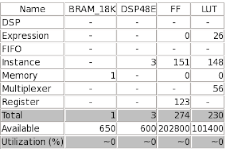
\includegraphics[scale=1.2]{lefttable}
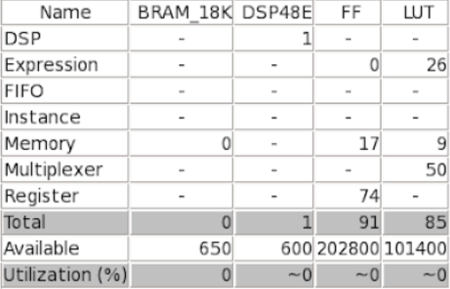
\includegraphics[scale=0.62]{righttable}
\caption{Results before on the left, results after on the right.}
\label{resulttable}
\end{figure}

Next, the test-bench was modified to calculate the RMSE between the software and simulated custom precision hardware implementation. This is useful in terms of understanding how accurate the implementation can be. (Code is in Appendix A.1)

\begin{figure}[h]
\centering
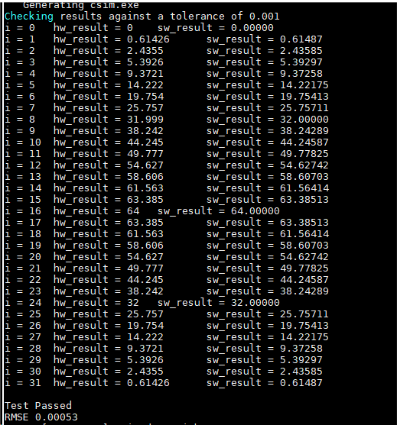
\includegraphics[scale=1]{RMSE}
\caption{Output of the simulation with RMSE code}
\label{RMSE}
\end{figure}




\section{ Design of a dot-product module}
The group were next tasked in designing a hardware module in Vivado HLS, which calculates the dot-product of two vectors. The module takes as input the two vectors in an array form and outputs the dot-product as an integer. This function is called upon by the test bench (displayed in the appendix), and compares the output with the expected answer calculated by the software. When the group tested this, an unroll factor was used to optimise the hardware. “Unrolling” the code is a term describing the process of repeating the blocks required for this function to reduce the number of iterations or “trips” of the loop required. \cite[p.321]{crockettelliottenderwitzstewart2014} Therefore, instead of using the same hardware over and over, the code can send data concurrently to the hardware, in turn reducing the latency of the system and increasing the throughput. Looking at the table below, an observation can be made showing that increasing the unroll factor causes more use of hardware, but decreases the throughput. In this task, the group chose the array size to be 10, so the loop had to run only 10 times, therefore an unroll factor of 10 has fully unrolled the loop making the most of the pipelining and also making the hardware more complex. An unroll factor higher than that for this task would make no difference, as the loop is fully unrolled.


\begin{figure}[h]
\centering
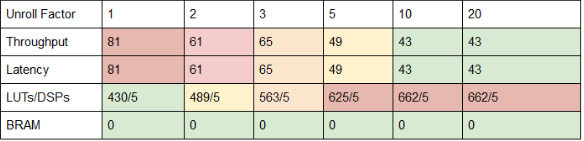
\includegraphics[scale=1]{unrolltable}
\caption{Comparison of effect of different unroll factors}
\label{unrolltable}
\end{figure}


\section{Creating a program to interact with Overlay on the PYNQ board.}

In the next task, the team was introduced to the actual PYNQ board. The group were given instructions on how to connect and set up the PYNQ board and use the Jupiter environment to compile and upload python to the CPU. Jupiter’s Edit and Command mode allow testing of  individual cells, making organizing and debugging much more efficient. The python software scripts written in the Jupyter Notebook interact with PYNQ’s programmable logic (PL) by running on its processing system (PS) via the AXI interface.\cite[p.6]{crockettelliottenderwitzstewart2014}

The task was to create a binary counter (code in the Appendix A.4). For debugging purposes the team made some code for service LEDs to flash when the code is uploaded. The team has also decreased the timing between each individual count.


\section{Overlay design}

The next task on the PYNQ board that the team tackled was to create a number adding program (See the appendix for code). Once again, a Vivado HLS with the “NumAdd” C code and needed directives was created. All inputs and outputs have been set to Slave lite interface so that they could communicate with the CPU\cite[p.299]{crockettelliottenderwitzstewart2014}. Running the synthesis to convert into HDL showed that the addition was implemented using LUTs instead of DSPs. 

The next step was to add an HDL wrapper to the design and generate the bitstream, allowing it to be used for the PL on the PYNQ board. In the end, the team has generated the .tcl file, containing the project block diagram. PYNQ board uses the tcl script to identify the configuration system and IP data such as control signals, for interface with the PS.
The final step was to record the address data for the overlay ports so that the PS would know how to reference the read/write ports of the block. The address attributed to the block was at the offset of 0x43C0\_0000 with the highest address of 0x43C0\_FFFF and range of 64k. Then, the team also recorded the address of the inputs and outputs inside the block, which were 0x00 for the control signals, 0x10 for signal a, 0x18 for signal b and 0x20 for signal y.  The data signals were predefined in the C code as 32-bit data ports.

In the final step, the custom overlay, which is used for file creation on the PYNQ FPGA and MMIO were loaded onto the PYNQ board and interfaced via different classes. 

To manage the communication with the PL, the group has used control signals such as ap\_start. This triggers blocks calculation and ap\_done, which in turn allows the team to get feedback when the results are ready to be read. There are other control signals that could be used such as ap\_ready (when the block is ready for the new input) and ap\_idle, which indicates if the block is operating or currently idle\cite[p.303]{crockettelliottenderwitzstewart2014}. The code has been adjusted to allow the calculation to take more than one cycle, via the use of ap\_done, before reading the output.


\section{Starting with PYNQ Video Processing and Computer Vision Reference Design.}

The team started with sending the HDMI signal through the PYNQ board the team got 60FPS. However, when turned on grayscaling the FPS dropped significantly to below 10FPS, which was expected, but not to this extent.

The next step was to move onto edge detection algorithms, as the tutorial sheet suggests. The given code imports an image and performs edge detection on it and saves it as a new file (See Figure \ref{edgedetection}). The C Synthesis estimated the following hardware usage (See table \ref{ResourceUse}). Since the dimensions of the image are undefined at execution time, there is no latency prediction in the synthesis. By redefining the image size, the number of loop executions and hence the timing can be estimated. The team synthesised the hardware block design in Vivado. Shown below are the hardware resources needed in the actual design. There is a noticeable increase in resource usage, due to the fact that Vivado HLS only gives value for the block designed, while Vivado adds all the interface and integration blocks in order for the PL and PS to function together. 

\begin{figure}[h]
    \centering
    \begin{subfigure}[b]{0.6\textwidth}
        \centering
        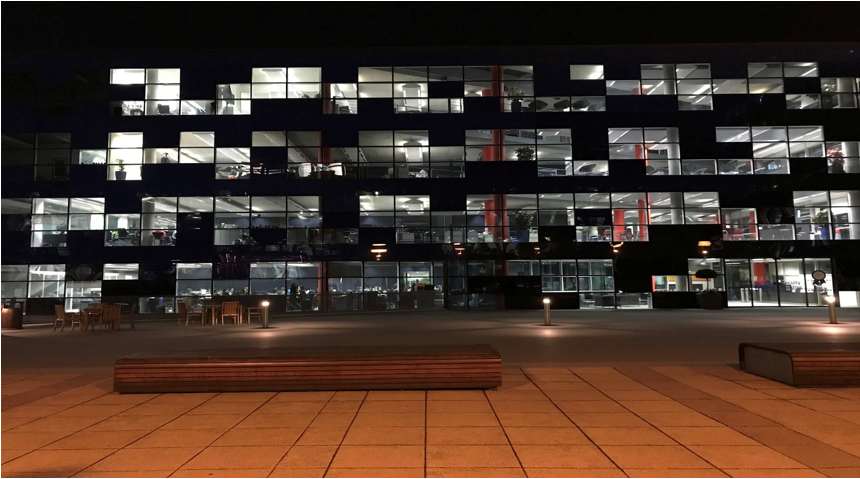
\includegraphics[width=\textwidth]{beforefilter}
        \caption{Initial image}
        \label{beforefilter}
    \end{subfigure}
    \begin{subfigure}[b]{0.6\textwidth}
        \centering
        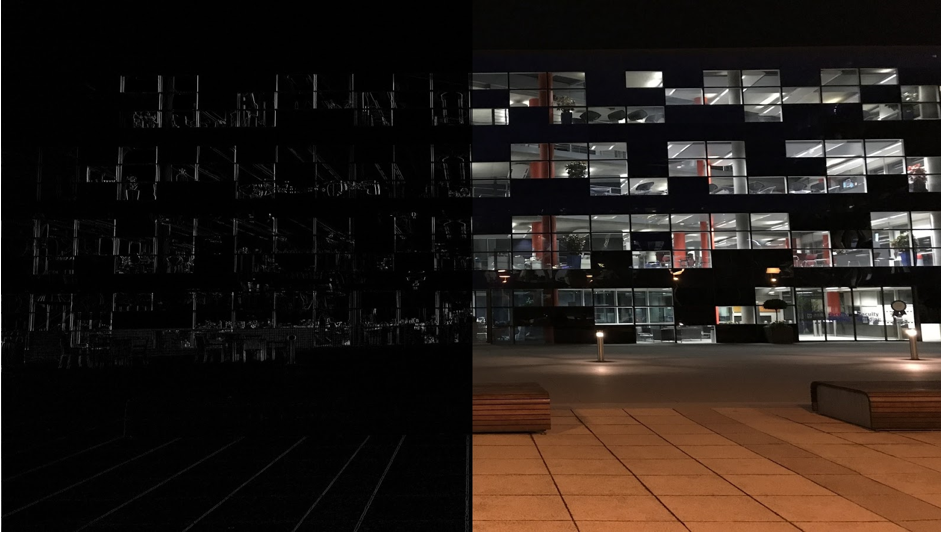
\includegraphics[width=\textwidth]{afterfilter}
        \caption{Half the image edge detected}
        \label{afterfilter}
    \end{subfigure}
    \hfill
    \caption{Demonstration of edge detection on half the image}
    \label{edgedetection}
\end{figure}


\begin{table}[h]
\centering
\begin{tabular}{ |p{3cm}||p{2cm}|p{2cm}|p{2cm}|p{2cm}|}
 \hline
 SOFTWARE & BRAM\_18K & DSP48E & FF & LUT\\
 \hline
 \hline
 Vivado HLS   & 2 & 13 &  3841 & 5809\\
 Vivado & 64 & 31 & 61462 & 40028 \\
 \hline
\end{tabular}
\caption{Comparison of resource use between Vivado HLS and Vivado.}
\label{ResourceUse}
\end{table}

\section{Modifying the design to add Horizontal Edge detection.}

The final step was to implement horizontal edge detection. If one would just rewrite the vertical edge detection code, changing the horizontal and vertical variables, the design would be extremely inefficient since the “in\_data” pointer would have to jump around in the memory. This is the case since the data of the image is stored in such a way, that once the pointer is incremented it points to the next pixel on the x-axis, but not on the y-axis. Hence, the group decided to use a buffer that stores the grey values of the whole previous row, for which they used an array with the image width as its predefined size (and further predefined the image width and height). Calculating the difference between each “grayscale pixel” from the current and the last row thus avoids the jumping (see code in the appendix A.5). For output of the program see Figure \ref{horizontaledge}.


\begin{figure}[H]
\centering
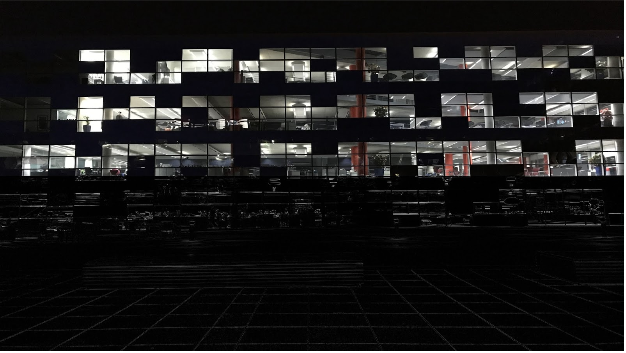
\includegraphics[scale=0.8]{horizontaledge}
\caption{Horizontal edge filter output}
\label{horizontaledge}
\end{figure}

Both the vertical and horizontal edge detection algorithms require approximately the same amount of hardware apart from BRAM (see Table \ref{ResourceUseEdge}). This can be traced back to the extra array the horizontally operating algorithm uses.

\begin{table}[H]
\centering
\begin{tabular}{ |p{3cm}||p{2cm}|p{2cm}|p{2cm}|p{2cm}|}
 \hline
 SOFTWARE & BRAM\_18K & DSP48E & FF & LUT\\
 \hline
 \hline
 Vertical   & 2 & 13 &  3841 & 5809\\
 Horizontal & 6 & 13 & 4248 & 5795 \\
 \hline
\end{tabular}
\caption{Comparison of resource use between Vertical and Horizontal edge detection filters.}
\label{ResourceUseEdge}
\end{table}









\chapter{Project}
\section{Overview}
The team has been set with a task to design and make a project based on the PYNQ board that would process a camera input in real time and use that as an input into an interactive application. The group has decided that creating a game, with the purpose of entertaining the user would be the best idea. 

The team started exploring different approaches to this task. One of the initial ideas was to make a game similar to Draw with friends, where it flashes a word and the person has to draw the word, while the other person is guessing. After some consideration, the group has decided against that idea because it would require very careful hand motion tracking, which would be complex.

	In the end, the decision has been made to go with a game, which the team called “CookEIE monster”. The idea of the game is to catch cookies with your mouth and avoid broccoli. The player will have 3 lives and if he comes into contact with broccoli, life would be lost. When the life counter reaches 0, the game is over. A player can restart the game at anytime by covering the camera completely.


The goals for this project would be:
\begin{itemize}
  \item Produce a python game interface
  \item Use object recognition techniques to detect a mask (which would be worn by the player on their face, so that the system could detect it).
  \item If the previous step is successful, extend the capabilities to detecting a face and if the mouth is open or not.
  \item The output FPS to be no lower than 24.
\end{itemize}

\section{High level overview}


Each frame, the camera output is being stored into an image buffer on the PYNQ board’s RAM. The FPGA will access and analyse this data, outputting two integer coordinates and one boolean value. The procedure in the FPGA can be divided into two main parts: Processing and Detection. 

All the algorithms in this section were implemented in Javascript as a proof of concept (see Appendix A.6 for code).

First, using multi-level thresholding\cite{resma2018multilevel}, the group wants to separate pixels that fall in a predefined colour range by making them white (Hex FFFFFF) while making all other pixels black (Hex 000000) (see figure \ref{edge detection}).



\begin{figure}[h]
\centering
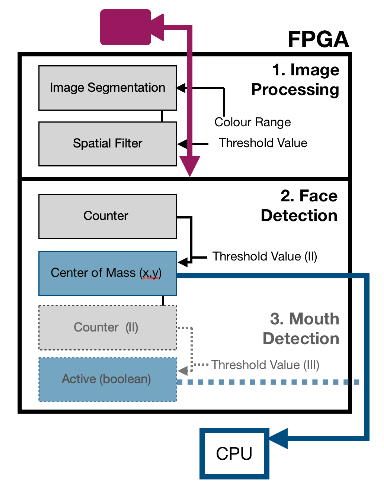
\includegraphics[scale=1]{schematic}
\caption{Block diagram of the project.}
\label{schematic}
\end{figure}

\begin{figure}[H]
    \centering
    \begin{subfigure}[b]{0.45\textwidth}
        \centering
        
\includegraphics[width=\textwidth]{chrispre}
        \caption{Pre processing.}
        \label{chrispre}
    \end{subfigure}
    \hfill
    \begin{subfigure}[b]{0.45\textwidth}
        \centering
        
\includegraphics[width=\textwidth]{chrispost}
        \caption{Post processing.}
        \label{chrispost}
    \end{subfigure}
    \hfill
    \caption{Face detection algorithm.}
    \label{edge detection}
\end{figure}


To get the right colour range, the group sampled multiple skin tones under different light conditions, producing the following range: (see Figure \ref{colorrange})

\begin{figure}[H]
\centering
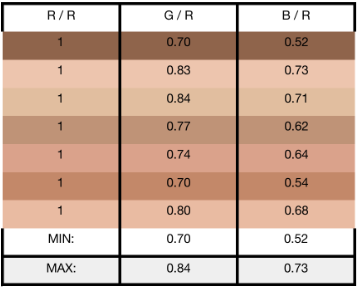
\includegraphics[scale=1]{colorrange}
\caption{Ratio of green and blue RGB values to red for different skin tones.}
\label{colorrange}
\end{figure}

The table shows the ratios of the green and blue values compared to the red value of each sample. By looking at the ratio range of RGB values instead of the range of each RGB colour, the group hopes to minimize problems concerning the light condition and thus achieve more accurate thresholding.

Next, a spatial filter\cite{nguyen2012} will be applied in order to minimize the number of white pixels in the background. This can be done by locating the neighbours of each white pixel, presumably in sizes of 3x3\cite[p.12]{nelson}, and changing all pixels in that group to black if the amount of white pixel is below a threshold of 50\%. As with all predefined values in this description, this threshold value will likely be adapted during testing.

Since groups of one pixel now have the same colour, the image resolution could possibly be decreased by a factor of 9 so that would result in a better performance. Furthermore, both thresholding and the spatial filter could be combined by only making a pixel white if 50\% of its neighbours are in the defined colour range (see Figure \ref{threshold}).


\begin{figure}[H]
    \centering
    \begin{subfigure}[b]{0.45\textwidth}
        \centering
        
\includegraphics[width=\textwidth]{img1}
        \caption{Below threshold.}
        \label{below}
    \end{subfigure}
    \hfill
    \begin{subfigure}[b]{0.45\textwidth}
        \centering
        
\includegraphics[width=\textwidth]{img2}
        \caption{Above threshold.}
        \label{above}
    \end{subfigure}
    \hfill
    \caption{Spatial filter example.}
    \label{threshold}
\end{figure}

In the second stage, a counter counts all the white pixels and decides if a face is present or not by comparing it to a predefined threshold\cite[p.23]{inproceedings}. If that threshold is surpassed, the centre of mass of all white pixels is calculated, detecting the face of the player and returning its x and y value. 

\begin{figure}[H]
\centering

\includegraphics[scale=1]{final1}
\caption{Calculated center of mass represented with red square.}
\label{schematic}
\end{figure}

The final step the group considers is detecting the mouth of the player. This could be done by finding the height of the black cluster underneath the centre of the face. If that height is bigger than a predefined threshold, the function returns true, else wise it returns false.

\section{Expected Outcome}

The team by the end of the project aims to have achieved a system which recognises the player's mouth to play the game. For this to happen first the code for face detection has to be made, and from there the team can move onto recognizing the mouth of the player. With that, all completed to a high standard, where the frame rate is high and the recognition works all the time, the signal can then be processed by the CPU. In this, the python code should be able to create a game of falling cookies after the camera has been turned completely black, which would indicate a restart for the game. Here when the cookies fall the signal from the image processing unit should be used as input. When the cookies touch the hitboxes of the mouths, they will be “eaten”. The player will need to avoid falling broccoli, otherwise would lose a life. When all the 3 lives have been lost the game is over.  All of this should happen in real time to keep in line with the specification. To end the game, the black card should be brought in front of the camera again. 

	Initially, the team will only use a ‘Cookie Monster’ mask. This should be easily recognisable due to the blue colouring. If this works well, a step can be taken to move this down to the mouth. At first, this will just a be a hitbox, so no matter if the mouth is open or closed, the hitbox will still be there. Therefore, the overall aim of the project is to make the hitbox on the mouth and to make it disappear if the mouth is closed. If this is successful, this could be extended to 2 players. In the top corner of the game will be the player's score, 1 point per cookie. In the top left will be the lives the player is one. Each player starts with 3 lives. 

	Another aspect of the game the team wants to achieve is having the sprites fall at different speeds. This will add a level of difficulty to the game. As the game goes on the faster on average each item will fall. Below is a crude diagram of the final UI design of the game (see Figure \ref{UI}). 


\begin{figure}[h]
\centering

\includegraphics[scale=1]{UI}
\caption{Sketch of the UI of the game.}
\label{UI}
\end{figure}

\section{Project Planning}

With 60 days left on the project, The team have filled their time wisely with the Gantt chart pictured below (see Figure \ref{gantt}). When planning out the project they have distributed the focus throughout the group, playing to individual strengths in the area. One can see this more clearly by observing the key next to the Gantt chart (see Figure \ref{ganttkey}) showing; Edward Harriss will be focused on python (making the game), Christoph Renschler will be focused on the C code (detection of objects than later on the face), and Nikita Belenkov will be focused on hardware usage (optimising the project to hit the minimum 24FPS performance).

	In the week leading up to the holidays, each member of the team will research their respected area. This is so the team can start the coding as soon as possible over the holidays. In the long run, this will stop the backlog of work during term time and allow the team to optimise the code better once all of the members are together. The team believes this is the best solution to make better use of our time. It also allows plenty of time to troubleshoot any major and minor errors that the team will come across.

	Once the team has regathered from the holidays, they will meet up and start optimisation and testing. This will last a week. The reason behind this decision is simple: on presentation day, the team wants to put forward their best work which works fully with very limited bugs. Also from experience of the group, on big projects like this, a lot of bugs need to be ironed out before the submission.

	One may have observed from the Gantt chart the final project spans 55 days throughout the holiday. This is so while the team is working upon the project they can collect ideas and take notes. Once the project is completed a week before the deadline, the team can arrange their ideas and notes into a report and presentation. Overall the team believes this is the best strategy to perform with the complexity of this project. 


\begin{figure}[H]
    \centering
    \begin{subfigure}[b]{0.25\textwidth}
        \centering
        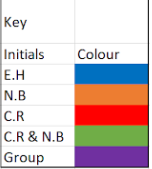
\includegraphics[width=\textwidth]{key}
        \caption{Colour key.}
        \label{key}
    \end{subfigure}
    \hfill
    \begin{subfigure}[b]{0.7\textwidth}
        \centering
        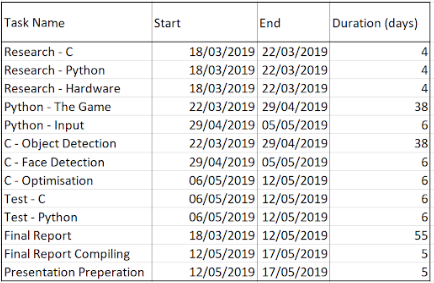
\includegraphics[width=\textwidth]{key1}
        \caption{Gantt Breakdown}
        \label{key1}
    \end{subfigure}
    \hfill
    \caption{Gantt chart explanation.}
    \label{ganttkey}
\end{figure}

\begin{figure}[h]
\centering
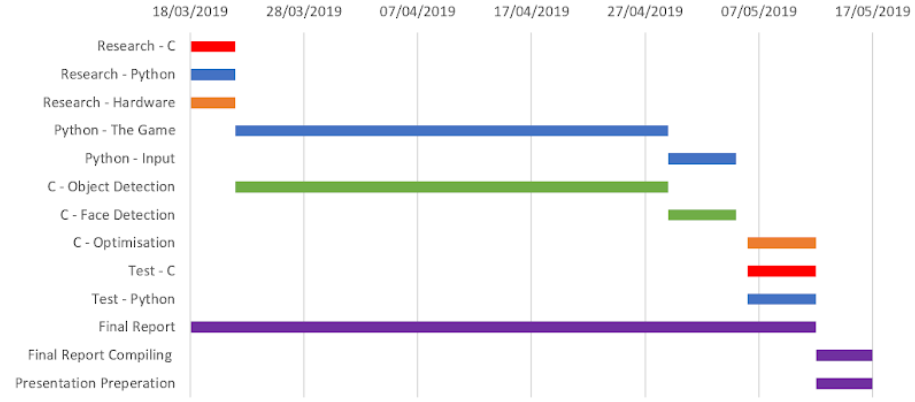
\includegraphics[scale=0.6]{gantt}
\caption{Planned gantt chart}
\label{gantt}
\end{figure}






\chapter{Conclusion}
Overall, based on the knowledge acquired from the work on the tutorials and labs in the past few weeks and the past and future research, the team believes that this is an optimal project, because it allows for the team to utilize the board to its limits and make something that the group would find both interesting, challenging and unique. Planning has been taken seriously, because the time is limited and the possibility of things going wrong is very high, so many levels of the project has been introduced, such as starting with the mask, if that works moving to face detection and if that works moving to mouth detection. This strategy allows having a working product, which could be showcased, at most stages of the project, which the team believes is extremely important.

\appendix
\chapter{Appendix}
\section{RMSE calculation code}
\lstset{language=C++}
\begin{lstlisting}
#include <iostream>
#include <iomanip>
using namespace std;

#include "window_fn_top.h"

#ifdef FLOAT_DATA
#define ABS_ERR_THRESH 0.0
#else
#define ABS_ERR_THRESH 0.001
#endif

#define WINDOW_FN_DEBUG 1

int main(void)
{
   win_fn_in_t testdata[WIN_LEN];
   win_fn_out_t hw_result[WIN_LEN];
   float sw_result[WIN_LEN];
   unsigned err_cnt = 0;

   // Generate test vectors and expected (real valued) results
   for (int i = 0; i < WIN_LEN; i++) {
      float samp_i = 64.0;
      // Use the coefficient calculation function from class for convenience
      float win_i = xhls_window_fn::coef_calc<WIN_LEN,WIN_TYPE>(i);
      testdata[i] = samp_i; // implicit conversion from float to ap_fixed<>
      sw_result[i] = samp_i * win_i; // generate floating point expected values
   }

   // Run the DUT
   window_fn_top(hw_result, testdata);

   // Check results
   cout << "Checking results against a tolerance of " << ABS_ERR_THRESH << endl;
   cout << fixed << setprecision(5);
   float sum = 0;
   int count = 0;
   for (unsigned i = 0; i < WIN_LEN; i++) {
      float abs_err = float(hw_result[i]) - sw_result[i];
      sum += abs_err * abs_err;
      count ++;

#if WINDOW_FN_DEBUG
      cout << "i = " << i << "\thw_result = " << hw_result[i];
      cout << "\t sw_result = " << sw_result[i] << endl;
#endif
      if (fabs(abs_err) > ABS_ERR_THRESH) {
         cout << "Error threshold exceeded: i = " << i;
         cout << "  Expected: " << sw_result[i];
         cout << "  Got: " << hw_result[i];
         cout << "  Delta: " << abs_err << endl;


         err_cnt++;
      }
   }
   cout << endl;

   // Print final status message
   if (err_cnt) {
      cout << "!!! TEST FAILED - " << err_cnt;
      cout << " results out of tolerance." << endl;
   } else{
      cout << "Test Passed" << endl;
   }
   // Only return 0 on success
   cout << "RMSE " << sqrt(sum/count) << endl;
   return err_cnt;
}


\end{lstlisting}

\section{Dot-Product calculation code}
\lstset{language=C++}
\begin{lstlisting}


#include "fir.h"

void dotProduct(
    data_t x[N],
    data_t y[N],
    data_t *output
) {
    data_t acc = 0;
    int i;
    Multloop: for(i=0; i < N; i++) {
#pragma HLS UNROLL factor=20
        acc += y[i]*x[i];
    }
    *output = acc;
}


\end{lstlisting}

\section{Dot-Product test bench}
\lstset{language=C++}
\begin{lstlisting}

#include <stdio.h>
#include <math.h>
#include "fir.h"

int main () {
  FILE         *fp;

  data_t signal, output;
  data_t progout = 0;
  data_t x[N] = {5, 7, -3, -4};
  data_t y[N] = {-2, 3, -5, 6};

  int i;
  
  fp=fopen("out.dat","w");

  dotProduct(x,y,&output);

  for (i=0;i<=N;i++) {
      progout = progout + (x[i]*y[i]);
  }

  fprintf(fp, "%i %i\n", progout, output);
  fclose(fp);
  
  printf ("Comparing against output data \n");
  if (system("diff -w out.dat out.gold.dat")) {

    fprintf(stdout, "*******************************************\n");
    fprintf(stdout, "FAIL: Output DOES NOT match the golden output\n");
    fprintf(stdout, "*******************************************\n");
     return 1;
  } else {
    fprintf(stdout, "*******************************************\n");
    fprintf(stdout, "PASS: The output matches the golden output!\n");
    fprintf(stdout, "*******************************************\n");
     return 0;
  }
}

\end{lstlisting}

\section{Python binary counter}
\lstset{language=Python}
\begin{lstlisting}
from time import sleep
from pynq.overlays.base import BaseOverlay

base = BaseOverlay("base.bit")

Delay1 = 0.3
Delay2 = 0.1
color = 0
rgbled_position = [4,5]

for i in range(7):
    for led in rgbled_position:
        base.rgbleds[led].write(i)
        base.rgbleds[led].write(i)
    sleep(Delay2)

for led in base.leds:
    led.on()    
while (base.buttons[3].read()==0):
    if (base.buttons[0].read()==1):
        color = (color+1) % 8
        for led in rgbled_position:
            base.rgbleds[led].write(color)
            base.rgbleds[led].write(color)
        sleep(Delay1)
        
    elif (base.buttons[1].read()==1): # LEDS Count-Up
        for n in range(16):
            for j in range(4):
                base.leds[j].off()
                
            if (n >= 8):
                base.leds[3].on()
                n -= 8
            if (n >= 4):
                base.leds[2].on()
                n -= 4
            if (n >= 2):
                base.leds[1].on()
                n -= 2
            if (n ==1):
                base.leds[0].on()
            sleep(Delay1)
            
        for j in range(4):
                base.leds[j].off()
            
    elif (base.buttons[2].read()==1):
        for led in reversed(base.leds):
            led.off()
        sleep(Delay2)
        for led in reversed(base.leds):
            led.toggle()
            sleep(Delay2)                  
    
print('End of this demo ...')
for led in base.leds:
    led.off()
for led in rgbled_position:
    base.rgbleds[led].off()
\end{lstlisting}

\section{Horizontal Edge Detection}
\lstset{language=C++}
\begin{lstlisting}
#include <ap_fixed.h>
#include <ap_int.h>
#include <stdint.h>
#include <assert.h>

typedef ap_uint<8> pixel_type;
typedef ap_int<8> pixel_type_s;
typedef ap_uint<96> u96b;
typedef ap_uint<32> word_32;
typedef ap_ufixed<8,0, AP_RND, AP_SAT> comp_type;
typedef ap_fixed<10,2, AP_RND, AP_SAT> coeff_type;

struct pixel_data {
    pixel_type blue;
    pixel_type green;
    pixel_type red;
};


void template_filter(volatile uint32_t* in_data, volatile uint32_t* out_data, int w, int h, int parameter_1){
#pragma HLS INTERFACE s_axilite port=return
#pragma HLS INTERFACE s_axilite port=parameter_1
#pragma HLS INTERFACE s_axilite port=w
#pragma HLS INTERFACE s_axilite port=h

#pragma HLS INTERFACE m_axi depth=2073600 port=in_data offset=slave // This will NOT work for resolutions higher than 1080p
#pragma HLS INTERFACE m_axi depth=2073600 port=out_data offset=slave


    int row [1920] = {0}; 

    for (int y = 0; y < h; ++y) {

        for (int x = 0; x < w; ++x) {

            #pragma HLS PIPELINE II=1
            #pragma HLS LOOP_FLATTEN off

            unsigned int current = *in_data++;

            unsigned char in_r = current & 0xFF;
            unsigned char in_g = (current >> 8) & 0xFF;
            unsigned char in_b = (current >> 16) & 0xFF;

            unsigned char out_r = 0;
            unsigned char out_b = 0;
            unsigned char out_g = 0;

            if (y>h/2){
                float curr_gray = 0.2126f*in_r  + 0.7152f*in_g  + 0.0722f*in_b ;
                int Y= abs(int(curr_gray)-row[x]);
                row[x] = curr_gray;

                out_r = Y;
                out_b = Y;
                out_g = Y;

            }
            else{
                out_r = in_r;
                out_g = in_g;
                out_b = in_b;
            }

            unsigned int output = out_r | (out_g << 8) | (out_b << 16);
            *out_data++ = output;

        }

    }

}

\end{lstlisting}

\section{Javascript code for simple colour detection using the p5.js library.}
\lstset{language=Java}
\begin{lstlisting}

var video, x, y, r, g, b, index, wr,wg,wb, slider;

function setup() {
 createCanvas(640, 480)
 pixelDensity(1);
 video = createCapture(VIDEO);
 video.size(width, height);
 slider = createSlider(0,1,0.1,0.05);
 slider.position(width/1.4,height/1.2);
 slider.style('width', '160px');

 mode = 1;
 
 wr = 1;
 wg = 223/255;
 wb = 196/255;//255,223,196
}


function draw() {
 video.loadPixels();
 //image(video, 0, 0);
 background(0);
 var val = slider.value();
 find(val);
}

function mouseReleased() {
  index = (mouseX + 1 + (mouseY * video.width)) * 4;
  wr = 1;
  wg = video.pixels[index + 1]/video.pixels[index + 0];
  wb = video.pixels[index + 2]/video.pixels[index + 0];
 console.log({wr,wg,wb});
}

function find(approx) {
 var tx = 0;
 var ty = 0;
 var counter = 0;
 for(y=0;y<video.height;y++) {
  for(x=0;x<video.width;x++) {
   index = (x + 1 + (y * video.width)) * 4;
   r = video.pixels[index + 0];
   g = video.pixels[index + 1];
   b = video.pixels[index + 2];
   
   if(abs(g/r-wg)<approx && abs(b/r-wb)<approx) {
    tx += x;
    ty += y;
    stroke(255)
    point(x,y);
    counter++;
   }
  }
 }
 tx /= counter;
 ty /= counter;
 noStroke();
 fill(255,0,0);
 //rect(tx,ty,50,50);
}

\end{lstlisting}

\bibliographystyle{IEEEtranN}
\nocite{*}
\bibliography{references}



\end{document}
